% !TEX root = ferguson-dissertation.tex

\chapter{Flowlog}

\section{Introduction}

In a software-defined network (SDN), switches delegate their control-plane
functionality to logically centralized, external controller applications.
This split provides several advantages including a global view of network
topology, and the use of general-purpose programming languages for implementing network polices.
These general-purpose languages require an interface
to the switch hardware, such as OpenFlow~\cite{McKeown:ccr08-openflow},
which also provides a basic abstraction of the switch's flow tables.

To best use this interface, recent research has produced domain-specific languages like
NetCore~\cite{monsanto:popl12-netcore} that can be proactively compiled to
flow tables. While this exclusive focus on flow tables simplifies compilation,
it hurts expressivity.
NetCore, for instance,
can describe a forwarding policy, but lacks the ability to reference (let alone
change) state on the controller.

Instead, the programmer must write a multi-tier program: a wrapper in a
general-purpose language that maintains control-plane state and dynamically creates new,
stateless data-plane policies to describe current forwarding goals. 
The data-plane policies must also specify
which packets the switches should send to the controller, but---due 
to the multi-tier, multi-language nature of these programs---there is no
structured connection between policies that describe packets the controller receives, and the arbitrary
code in a callback function that consumes them. This gap can lead to
bugs in how switches update the controller, resulting in incorrect
controller state or network policies. Moreover, if
packets are delivered to the controller needlessly, performance
suffers.

To better support controller programming, we have created \flowlog, a
\emph{tierless} network programming language. As in web-programming, where 
a program contains multiple tiers such as client-side JavaScript, a
server-side program, and a database, an SDN system also has multiple tiers:
flow rules on switches, a controller program, and a data-store for controller
state. By incorporating all of these tiers, a single, unified \flowlog\ 
program describes both control- and data-plane behavior.

\flowlog\ also provides built-in support for program verification. 
Because controller programs pose a single point of failure for the
entire network, verification tools
are invaluable to SDN developers. Prior SDN
controller analysis work has often focused on the switch rules themselves, either
statically~\cite{alshaer:safeconfig10-flowchecker,kazemian:nsdi12-hsa,mai:sigcomm11-anteater,reitblatt:sigcomm12-consistent-updates}
or dynamically, as each update is sent to the
switches~\cite{porras:hotsdn12-fortnox}. 
However, most SDN analyses focus on trace properties: statements
about the end-to-end behavior of packets in the network  (e.g., a lack of
routing loops). While these analyses are useful, they generally must be
performed with respect to a given topology, which 
limits their flexibility, reusability, and scalability. In contrast, our reasoning 
focuses on properties independent of network topology. 

%One subtle but important requirement for trustworthy
%static verification is sound reasoning about programs. However,
%reasoning about programs in
%languages as complex as Python~\cite{politz++:oopsla13-python} forces tough
%compromises between soundness and utility: preserving soundness requires
%performing so much over-approximation as to induce numerous
%false-positives. (This is in addition to well-understood decidability
%barriers induced by Turing-completeness.)
%Even compiler
%optimizations need soundness to maintain guarantees about program behavior across optimizations.
%Thus, soundness is a critical concern for
%both reliability and performance.

We have limited \flowlog's expressive power to support both tierlessness and
verification, while retaining enough expressivity to be useful for real-world
programming. A limited language poses obvious problems for
developers, both in expressing their needs and in reusing existing code.
\flowlog\ therefore provides interfaces and abstractions for
interacting with external programs. Programmers are free to invoke existing,
full-featured libraries as needed, depending on their analysis goals. This is
in contrast to most policy languages: in \flowlog, the restricted language
itself forms the primary program, calling the external code rather than being
called by it. This approach has been successful in SQL, where
database queries are in the ``limited'' language and user-defined functions are
in ``full'' languages. Our work explores such a strategy for network
programming. Our contributions are:
\begin{enumerate} 

\item{We present the tierless \flowlog\ language (\Cref{sec:syntax}) and
demonstrate its expressive power on real-world examples (\Cref{sec:examples}).
The language includes SQL-like relational state. It also provides abstractions
for interaction with external code, via either asynchronous \emph{events} or
synchronous \emph{remote tables}. \Cref{sec:impl} describes its
implementation.}

\item{We show how, in spite of \flowlog's tierless merging of data- and control-plane behavior, programs
can be proactively compiled to flow table rules (\Cref{sec:proactive}). The compilation process
extends beyond mere packet forwarding; it also filters packets that may trigger
state updates or cause event output and notifies the controller only as necessary.}

\item{We automatically compile \flowlog\ programs to the Alloy~\cite{jackson:alloybook} verifier
(\Cref{sec:analysis}). We focus on analyses that are
independent of network topology, which are especially helpful
when the topology is virtual, in flux, or unknown. 
We show that this process is aided by \flowlog's tierlessness as well as its limited expressiveness.
We are able to verify 
properties in less than a second with minimal developer input. This
verification support has helped us find surprising errors in our own
\flowlog\ programs.}

\end{enumerate}

%%%%%%%%%%%%%%%%%%%%%%%%%%%%%%%%%%%%%%%%%%%%%%%

\section{\flowlog\ by Example}
\label{sec:examples}

We introduce \flowlog\ with illustrative examples. These demonstrate
\flowlog's tierless nature, along with its expressive power, concision, and
ability to support real-world development needs. We have also designed
\flowlog\ to be amenable to both sound (\ie, no false positives) and complete 
(\ie, no bugs are missed) verification. To meet these goals, \flowlog\ bans
loops and recursion, and has a logical semantics that we leverage for sound
and, in many cases, complete verification (\Cref{sec:analysis}). Moreover, no
recursion means that \flowlog\ programs always terminate on each incoming event.

\paragraph{Stolen Laptop Detector}

Let us write an application to help campus
police track down stolen laptops. It must accept signals from campus
police that report a laptop stolen or recovered, and if a stolen
laptop is seen sending packets, the program must alert the police, saying which
switch the laptop is connected to and when the packet was seen. (For
brevity, we do not demonstrate rate limiting of alerts or restriction of alerts to edge-router traffic.
Both of these tasks can be accomplished in \flowlog.)

Without a tierless programming language, expressing this program would require
many pieces, possibly using multiple languages: a database or
data structures to manage controller state; a remote-procedure call (RPC)
library, or similar solution, for handling events; and policy-generation code
that produces fresh rules on the switches that forward traffic and check for
stolen laptops on the network. In \flowlog, all of these components share the
same abstraction. Suppose we have a table \fl{stolen} that tracks the MAC
addresses of all currently stolen laptops. Then, the heart of the program is
just the following rules:
\begin{lstlisting}[label=list:1]
ON stolen_report(sto):
  INSERT (sto.mac) INTO stolen;
ON stolen_cancel(rec):
  DELETE (rec.mac) FROM stolen;
ON packet_in(p): 
  DO notify_police(sto) WHERE 
    sto.mac = pkt.dlSrc AND 
    sto.time = time AND 
    sto.swid = pkt.locSw AND
    stolen(pkt.dlSrc) AND 
    get_time(time);    
  DO forward(new) WHERE 
    new.locPt != p.locPt;    
\end{lstlisting}
The program describes several kinds behavior that appear disparate. It: (a)
adds addresses to a table when laptops are reported stolen (lines 1--2); (b)
removes addresses when laptops are recovered (lines 3--4); (c) notifies police
when a packet appears from a stolen laptop (lines 5--11); and (d) floods packets (lines 12--13); 
this trivial example of forwarding introduces syntax which we will use later. With \flowlog's tierless abstraction,
we express all of this in four concise rules.

Every program has similar rules that describe how to handle each packet;
these rules are written in a syntax reminiscent of SQL, and the semantics is
correspondingly relational. In addition, most programs will have state that
must be updated in reaction to packets and other stimuli.  These stimuli are
external events, whose implementations can be arbitrary, and whose interfaces
are explicitly declared or built in. We now describe the program declarations
that support these rules. (Figure~\ref{fig:events} shows the different
components of \flowlog.)

\begin{figure}
  \centering
  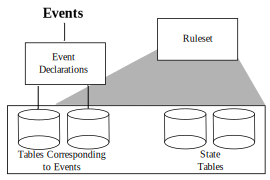
\includegraphics[scale=0.95]{figs/events-and-db.pdf}
  \caption{\small \flowlog\ system diagram. Events are represented by tuples
  in event tables. Rules interact with the entire database.}
  \label{fig:events}
\end{figure}

We have already seen \fl{stolen}, 
the internal controller state.
We expose the current time with an
external table \fl{get_time} (which always contains just one entry):% \\
\noindent
%\begin{minipage}{\linewidth}
\begin{lstlisting}[label=list:2]
TABLE stolen(switchid); 
REMOTE TABLE get_time(int); 
\end{lstlisting}
%\end{minipage}
External tables are managed by arbitrary external programs; in our examples,
we used OCaml programs running on the controller machine. Each table
declares its type, which is used for error-checking and optimization.

Next, we define the shape of incoming and outgoing events. We must
handle two kinds of notifications from the police, and send them one:
\begin{lstlisting}[label=list:3]
EVENT stolen_report {mac: macaddr};
EVENT stolen_cancel {mac: macaddr};
EVENT stolen_found {mac: macaddr, swid: switchid, time: int};
\end{lstlisting}
\flowlog\ processes incoming events one at a time.
Incoming events are placed in an identically named table,
causing dependent rules to be re-evaluated.
Outgoing events are also represented as
tables, and when the ruleset adds a tuple to such a table, \flowlog\ sends
an event with the tuple's content. 
These tables are therefore similar to named pipes in Unix. We require one such named pipe to
send \fl{stolen_found} events to the police server:
\begin{lstlisting}[label=list:4]
OUTGOING notify_police(stolen_found)
  THEN SEND TO 127.0.0.1:5050;
\end{lstlisting}
If a
\flowlog\ program inserts tuples into the \fl{notify\_police}
table, these tuples will be transformed into \fl {stolen\_found}
events and sent to a process listening on \fl{127.0.0.1:5050}. 
Incoming \fl{stolen\_report} and \fl{stolen\_cancel} events are
automatically inserted into their identically named tables. For
instance, the \fl{stolen_report} table will contain arriving
\fl{stolen_report} events, and the \fl{packet_in} table will hold incoming packets.
Notice we did not declare an outgoing \fl{forward} table. This is
because \flowlog\ automatically creates outgoing tables for common
packet-handling behavior, as detailed in Table~\ref{tab:built-in}.

The remote table \fl{get\_time} is populated by querying
\fl{127.0.0.1:9091}, and should be refreshed every second:
\begin{lstlisting}[label=list:5]
REMOTE TABLE get_time 
  FROM time AT 127.0.0.1:9091
  TIMEOUT 1 seconds;
\end{lstlisting}
The \fl{TIMEOUT} field (line 3) is vital for performance and correct proactive compilation. 
A numeric timeout gives a window during which the results can be cached. \flowlog\ also provides a \fl{NEVER} 
keyword, meaning the external callout has no side-effects, and thus its results can
be cached indefinitely. A default, empty timeout requires updating the remote table
every time the program is evaluated. 

The reader may wonder whether this program can be compiled to stateless rules and installed in switches. After all,
it contains a rule only the controller can handle, since
it involves notifying campus police. But this rule
only fires when \fl{stolen(p.dlSrc)} is true, so \flowlog's proactive
compiler instructs switches to send packets to the controller only if their
source-MAC field has been registered as stolen. Furthermore, \flowlog\ automatically
updates the switches every time a new theft is reported; no code to that effect is needed.

\begin{table*}
\small
\begin{tabular}{|l|l|l|}
\hline
\fl{INCOMING} {\bf Table}    & {\bf Corresponding \fl{EVENT} (with fields)}   & \bf{Description} \\
\hline
\fl{packet\_in}  & \fl{packet} \fl{\{locSw, locPt, dlSrc, dlDst, dlTyp, nwSrc, nwDst, nwProtocol\}} & packet arrival \\ 
\fl{switch\_port} & \fl{switch\_port} \fl{\{sw, pt\}}    & switch registration \\
\fl{switch\_down} & \fl{switch\_down} \fl{\{sw\}}  & switch down \\
\fl{E}            & \fl{E}                         & Any incoming event \fl{E} \\ 
\hline
\end{tabular}
\centering
\begin{tabular}{|l|l|l|}
\hline
\fl{OUTGOING} {\bf Table}      & {\bf Corresponding} \fl{EVENT} & {\bf Description} \\
\hline
\fl{emit}          & \fl{packet} & Emit a new packet \\
\fl{forward}       & \fl{packet} & Forward with modifications (triggered by packets only)  \\                   
\hline
\end{tabular}
\caption{\small Built-in \fl{INCOMING} and \fl{OUTGOING} tables. The \fl{locSw} and \fl{locPt} fields denote the packet's (switch and port) location.} 
\label{tab:built-in}
\hrule
\normalsize
\end{table*}

\paragraph{Network Information Base}
\label{sec:eg:nib}

Next, we show how \flowlog\ can be used to compute a network
information base, or NIB~\cite{koponen:osdi10-onix}. We begin with topology discovery, using \flowlog's
ability to process timer notifications and
emit new packets to run an LLDP-like protocol. First, we react to switch
registration to obtain identifiers for every port (omitting table declarations):
\begin{lstlisting}[label=list:6]
ON switch_port_in(swpt):
  INSERT (swpt.sw, swpt.pt) 
    INTO switch_has_port;
\end{lstlisting}
Thus, the \fl{switch\_has\_port} table will hold every
switch-port pair that registers. Next, we set up a
10-second event loop (we exclude the timer declaration):
\begin{lstlisting}[label=list:7]    
ON startup(empty_event):
  DO start_timer(10, "tNIB");
ON timer_expired(timer) 
  WHERE timer.id = "tNIB":
  DO start_timer(10, "tNIB");
\end{lstlisting}
The first rule uses \flowlog's built-in \fl{startup} event to start the
loop, and the second rule continues it. The constraint \fl{timer.id =
"tNIB"} accounts for situations where multiple timers may be in use.
The same timer also causes known switches to issue probe packets from each port:
\begin{lstlisting}[label=list:8]   
ON timer_expired(timer) 
  WHERE timer.id = "tNIB":
  DO emit(new) WHERE
    switch_has_port(new.locSw,new.locPt) 
    AND new.dlTyp = 0x1001
    AND new.dlSrc = new.locSw 
    AND new.dlDst = new.locPt;
\end{lstlisting}
We use \fl{dlTyp = 0x1001} (line 5) to mark probe packets. The
current switch and port IDs are smuggled in the MAC address fields of the
probe (lines 6-7). (We omit the rule that initiates the same probe emission
process on switch registration.)

We obtain knowledge of the switch topology from probe reception:
\begin{lstlisting}[label=list:9]   
ON packet_in(p) WHERE p.dlTyp = 0x1001:
  INSERT (p.dlSrc, p.dlDst,
          p.locSw, p.locPt) INTO ucST;
\end{lstlisting}
The table name \fl{ucST} denotes \emph{under
construction} switch topology; at any point, it contains a topology based on the
probes seen so far this cycle. We empty \fl{ucST} on every
cycle, and maintain a \fl{switchTopology} table that stores the value
of the last complete \fl{ucST} before it is deleted. \flowlog\ programs routinely use
this strategy of building up a helper table over an execution cycle,
separating in-progress results from the last complete result set:
\begin{lstlisting}[label=list:10]
ON timer_expired(timer) 
WHERE timer.id = "tNIB":
  DELETE (sw1,pt1,sw2,pt2) FROM ucST WHERE    
    ucST(sw1, pt1, sw2, pt2); 
  DELETE (sw1,pt1,sw2,pt2) 
    FROM switchTopology WHERE     
    switchTopology(sw1, pt1, sw2, pt2); 
  INSERT (sw1,pt1,sw2,pt2) 
    INTO switchTopology WHERE     
    ucST(sw1, pt1, sw2, pt2);  
\end{lstlisting}
Though \flowlog\ does not allow recursion (\Cref{sec:syntax}), 
we can use a similar approach to compute reachability on the network. This
program computes a fresh reachability table (\fl{ucTC}, for
under-construction transitive closure) as each probe arrives:
\begin{lstlisting}[label=list:11]   
ON packet_in(p) WHERE p.dlTyp = 0x1001
  AND dstSw = p.locSw AND srcSw = p.dlSrc:
  INSERT (srcSw, dstSw) INTO ucTC;
  INSERT (sw, dstSw) INTO ucTC 
    WHERE ucTC(sw, srcSw);
  INSERT (srcSw, sw) INTO ucTC 
    WHERE ucTC(dstSw, sw);
  INSERT (sw1, sw2) INTO ucTC 
    WHERE ucTC(sw1, srcSw) 
    AND   ucTC(dstSw, sw2);
\end{lstlisting}
The program works as follows: for every probe packet
received, it concludes that its source switch and its arrival switch
are connected (line 3). It also extends
existing reachability in both directions (lines 4--7). Finally,
it must account for packets connecting two cliques of reachability (lines
8--10).

It is instructive to compare this algorithm to the standard two-rule Datalog
program for transitive-closure~\cite[p. 274]{abiteboul.hull.ea:foundations}. The extra rules arise because we are \emph{not}
computing transitive-closure in the usual sense. Here, we do not have the luxury of
assuming that we possess the entire connection table in advance; we must
compute reachability on-the-fly as new information arrives. This difference
leads to added complexity. In fact, an initial version of this program lacked
the final rule, and so failed to faithfully compute reachability in some
cases; we found this bug using our verification tool (Section~\ref{sec:analysis}).

Once we have network reachability, we can compute a spanning
tree for the network:
\begin{lstlisting}[label=list:12]   
ON packet_in(p) WHERE p.dlTyp = 0x1001
  AND dstSw = p.locSw AND dstPt = p.locPt
  AND srcSw = p.dlSrc AND srcPt = p.dlDst:
  INSERT (srcSw, srcPt) INTO ucTree 
    WHERE NOT ucTC(srcSw, dstSw)
    AND   NOT ucTC(dstSw, srcSw); 
  INSERT (dstSw, dstPt) INTO ucTree 
    WHERE NOT ucTC(srcSw, dstSw) 
    AND   NOT ucTC(dstSw, srcSw); 
\end{lstlisting}
Again, we see unsurprising parallels to distributed
protocols. Ordinary spanning tree algorithms have the luxury of working with the
entire graph at once, and thus are often able to build a connected tree at
every step. We do not have that luxury here: probes may arrive in any order,
and we must build a forest of trees that, should links go down, may not even
be connected. We also must add a pair of rules, one for each direction of the
branch.
 
Of course, this spanning tree is not necessarily the best possible one; we
only compute the first such tree to be exposed by probe packets. Better
tree-generation algorithms can be written or accessed via external code.
Numerous other data, such as the location of connected hosts, can also be
gathered, but are omitted for space.

Given a spanning tree for the network---whether it is computed in \flowlog\ or
obtained from external code---we can construct a ``smart'' learning switch
application in \flowlog\ that does not suffer from the usual issues with cyclic
topologies. 

\paragraph{Other Examples} We have implemented additional applications
in \flowlog, which are available in our repository.\footnote{\url{http://cs.brown.edu/research/plt/dl/flowlog/}} These
examples include an ARP proxy, a stateful firewall, and an application
(which we use in-house) to facilitate access to Apple TV devices across subnets.

\section{The \flowlog\ Language}
\label{sec:syntax}

% In the criminal justice system, there are two separate but equally important...
% The ruleset is our Sam Waterston. 

As seen in Section~\ref{sec:examples}, every \flowlog\ program contains a
declarative \emph{ruleset} that governs controller behavior and a set of
\emph{declarations} for the program's state tables and incoming/outgoing interface.
Figure~\ref{fig:syntax} gives the concrete syntax of \flowlog\ rulesets.

%\emph{data-definitions} that intercept events, query the ruleset, and take appropriate action. These are augmented by 

% TN note: The commented-out BNF is _old_. Needs updating if we decide to use it.

%decl ::= event_decl | table_decl |
%         out_decl   | inc_decl;
%event_decl ::= EVENT <id> {listof(<id>)};
%table_decl ::= [REMOTE] TABLE <id> (listof(<id>));
%inc_decl ::= INCOMING <id> (listof(<id>));
%out_decl ::= OUTGOING <id> (listof(<id>));

%react_stmt ::= inc_defn | out_defn | remote_defn;
%remote_defn ::= REMOTE TABLE <id> FROM <id> 
%               AT <ip> <port> timeout;
%timeout ::= empty | TIMEOUT <num> | PURE;
%out_defn ::= OUTGOING <id> (listof(<id>)) THEN 
%             SEND EVENT TO <id> 
%             AT <ip> <port>;
%inc_defn ::= INCOMING <id> THEN INSERT INTO <id>;

\begin{figure}[t]
\footnotesize
\begin{verbatim}
block ::= ON <id> ( <id> ) [WHERE rformula] : rules
rules ::= rule | rule rules
rule  ::= do_act | ins_act | del_act
do_act  ::= DO <id> ( termlist ) [WHERE rformula] ;
ins_act ::= INSERT ( termlist ) INTO <id> [WHERE rformula] ;
del_act ::= DELETE ( termlist ) FROM <id> [WHERE rformula] ;
term ::= <num> | <string> | <id> | <id>.<id> | ANY
termlist ::= term | term , termlist
rformula ::= <id> ( termlist ) | term = term | NOT rformula | rformula AND rformula | 
             rformula OR rformula | ( rformula )   
\end{verbatim}
\normalsize
\caption{\small Syntax of \flowlog\ rulesets. A program is a succession of \fl{ON} blocks. Optional arguments are in square brackets. Capitalized tokens and punctuation are reserved constants.}
\label{fig:syntax}
\end{figure}

\paragraph{Declarations}

A program declares \fl{EVENT}s, state \fl{TABLE}s, and interfaces for
\fl{INCOMING} and \fl{OUTGOING} tables.  Most \fl{INCOMING} and some \fl{OUTGOING} 
declarations are made automatically when events are declared. Declaring a table as
\fl{REMOTE} informs \flowlog\ that the table represents a callout
to external code, and that the ruleset will not maintain that table's state. Every
event declaration is equipped with a set of field names for that event type.
Every internal table and interface table is equipped with a type, given as a vector
of type names (e.g., ``switchid'')---one for each column in the table.
\fl{REMOTE TABLE} and \fl{OUTGOING} declarations must also be provided with
additional information, as we saw in \Cref{sec:examples}.

%\paragraph{Reactive Subprograms}
%A reactive program concretizes a declared interface, connecting database 
%tables to the world of packets and
%events. Space restrictions prevent us from discussing the reactive program
%semantics in detail, but they query the ruleset to bridge between tables and 
%the real world where packets arrive. 

\paragraph{Rulesets}

\begin{figure*}
\small
\centering
\begin{tabular}{|l l|}
\hline
  \fl{ON IN(in) DO OUT(o1, ..., ok) WHERE rf}          & $\forall in,o_1,...o_k \; \exists e_1, ..., e_k \; OUT(o_1, ... o_k) \leftarrow IN(in) \wedge \RF(\mfl{rf})$\\
  \fl{ON IN(in) INSERT (o1, ..., ok) INTO R WHERE rf}  & $\forall in,o_1,...o_k \; \exists e_1, ..., e_k \; \addR(o_1, ... o_k) \leftarrow IN(in) \wedge \RF(\mfl{rf})$ \\
  \fl{ON IN(in) DELETE (o1, ..., ok) FROM R WHERE rf}  & $\forall in,o_1,...o_k \; \exists e_1, ..., e_k \; \delR(o_1, ... o_k) \leftarrow IN(in) \wedge \RF(\mfl{rf})$ \\
\multicolumn{2}{|c|}{(All rules existentially quantify variable occurrences that are free and not in $\{in, out_1, ..., out_k\}$; hence the $e_i$s.)} \\ 
\hline
\end{tabular}

\minipage{0.25\textwidth}
\begin{tabular}{|l l l|}
\hline
  $\RF(\mfl{NOT f})$           & $=$    & $\neg \RF(\mfl{f})$ \\
  $\RF(\mfl{f1 AND f2})$       & $=$    & $\RF(\mfl{f1}) \wedge \RF(\mfl{f2})$ \\
  $\RF(\mfl{t1 = t2})$         & $=$    &  $\TT(\mfl{t1}) = \TT(\mfl{t2})$\\  
  $\RF(\mfl{P(t1, ..., tk)})$  & $=$    & $\exists x_1, ..., x_k \; P(\TT(\mfl{t1}), ..., \TT(\mfl{tk}))$ \\
                               &        & \hphantom{m} $x_1$, ..., $x_k$ are the fresh variables introduced\\ 
                               &        & \hphantom{m} by \fl{ANY}s in the original formula. \\  
\hline
\end{tabular}
\endminipage\hfill
\minipage{0.32\textwidth}
\begin{tabular}{|l l l|}
\hline
  $\TT(\mfl{c})$     & $=$   & $c$ \\
  $\TT(\mfl{x})$     & $=$   & $x$ \\
  $\TT(\mfl{x.fld})$ & $=$   & $fld(x)$ \\
  $\TT(\mfl{ANY})$   & $=$   & $x_{fresh}$ \\
\hline
\end{tabular}
\endminipage
\normalsize\hfill

\caption{\small Rule-formula to formula ($\RF$) and Rule-term to term ($\TT$)
transformation functions. Without loss of generality, we provide every rule with its own
\fl{ON} trigger and assume that disjunction in rule bodies has been removed,
resulting in multiple rules. $x_{fresh}$ denotes a fresh variable.}
\label{fig:rule2formula}
\hrule
\end{figure*}

A ruleset contains a set of \fl{ON} blocks of rules. While we allow
multiple rules within the same \fl{ON} block for conciseness, without loss of
generality we will pretend that every rule has its own \fl{ON} block. Each
rule indicates an action to be taken when the \fl{ON}-specified trigger is
seen: either to \fl{INSERT} or \fl{DELETE} a tuple from the controller state,
or to \fl{DO} an action such as forwarding a packet. Finally, rules and triggers have an
optional \fl{WHERE} clause, which adds additional constraints; these are always an
expression involving only the tables declared in \fl{TABLE}s, never
those declared as \fl{INCOMING} or \fl{OUTGOING}. 
These rules determine a function that maps controller state and incoming
events to a new state and set of outgoing events.

Each rule defines a logical implication
stating that, should its body be satisfied, its action should be as well. 
Figure~\ref{fig:rule2formula} shows how we arrive at this \emph{rule clause} for each rule.
If the rule's action is \fl{DO}, then the resulting clause inserts tuples into the outgoing table directly. 
If the rule's action modifies an $n$-ary table $R$ via the \fl{INSERT} or \fl{DELETE} keywords, the clause
uses $n$-ary helper tables $\addR$ or $\delR$, which hold the tuples to be
added to and removed from the controller state after an event is processed.

If $\mdlS$ is a controller state, let $\mdlSplus$ represent the unique least expansion
of $\mdlS$ that satisfies all rule clauses. That is, while $\mdlS$ contains a table
for each \fl{TABLE}, $\mdlSplus$ also contains ephemeral $\addR$ and $\delR$
tables for each \fl{TABLE} as well as tables for each \fl{OUTGOING}
declaration. These \fl{OUTGOING} tables are consumed by \flowlog\ and dictate which outgoing events it should send. The ephemeral
tables for each state table $R$ dictate its value in the next state
as follows: 
\[R_{\mathit{next}} = (R^\mdlS \; \setminus \; \delR^{\mdlSplus}) \; \cup \; \addR^{\mdlSplus}\]
In other words, \fl{INSERT} overrides \fl{DELETE} in \flowlog---the next state's $R$ contains
the pre-state's $R$, minus $\delR$, plus $\addR$.

% END SYNTAX/SEMANTICS SECTION
%%%%%%%%%%%%%%%%%%%%%%%%%%%%%%%%%%%%%%%%%%%%%%%%%%%%%%%%%%%%%%%%%%%%

\section{Proactive Compilation for \flowlog}
\label{sec:proactive}

While \flowlog\ programs receive many kinds of input---both packets and
external notifications---packets remain the most common and time-sensitive
stimuli.  No software-defined network can scale to the level required by large
networks if it sends every arriving packet to the controller for instructions.
This complicates the implementation of a tierless SDN language; rather than
simply have all packets be processed by the controller in accordance with the
program, the \flowlog\ runtime is forced to solve three related, but distinct, 
challenges:

\begin{enumerate} 

\item{It must compile a program's \emph{forwarding behavior} to
equivalent OpenFlow~\cite{McKeown:ccr08-openflow} rules whenever possible,
including references to both local and remote state;}

\item{it must discern which packets can trigger non-forwarding
behavior, such as emission of an event or a state change, and produce
OpenFlow rules that send those packets---and only those packets---to the
controller; and,}

\item{if a rule uses features that are not supported by switch tables (we
detail these cases later), the compiler determines the class of packets
that must be sent to the controller for correct handling.
This situation applies to both
forwarding and non-forwarding rules.}

\end{enumerate}
As Section~\ref{sec:syntax} demonstrated, \flowlog\ rules can
involve equality between packet fields, negation, database state, and
numerous other features not supported by OpenFlow. Moreover, rules
can contain existentially quantified variables that, at first glance, require
searching and backtracking in the state to properly handle. Simply put,
\flowlog\ rules are strictly more powerful than OpenFlow 1.0 flow rules. It is
therefore reasonable to wonder: can a non-trivial amount of \flowlog\ really
be compiled faithfully? This section will show it can be.
Figure~\ref{fig:compilation} shows the compilation dataflow.

\begin{figure}
\centering
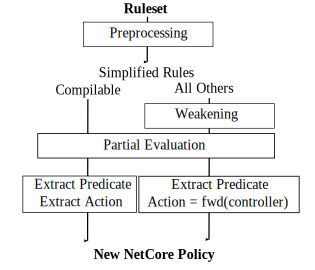
\includegraphics[width=2.5in]{figs/flowlog-compilation.pdf}
\caption{\small \flowlog's compilation process. Rules are first preprocessed before
being checked for compilability, then (if uncompilable) weakened before being
partially evaluated in the current state. After partial evaluation, the rule
is re-written as a stateless NetCore policy.}
\label{fig:compilation}
\hrule
\end{figure}

Our proactive ruleset compiler has three stages:
\begin{enumerate}

\item First (Section~\ref{sec:comp-preprocess}), it simplifies each rule
and identifies the compilable forwarding rules.
Both non-forwarding rules (state updates, emission of fresh packets,
etc.)\ 
and non-compilable forwarding rules require switches to
send packets to the controller; fortunately, these notifications can be extensively
filtered based on the program's structure.

\item Second (Section~\ref{sec:comp-partial}), it partially evaluates the ruleset at the current controller state, 
producing a new ruleset that has no references to state tables. Since the
original ruleset defines a function that accepts a state and an incoming tuple and
returns a set of outgoing tuples, the resulting ruleset depends only on the incoming tuple.

\item Finally (Section~\ref{sec:comp-policy}), it compiles the new ruleset automatically to flow table rules in two steps. 
First, it
converts to NetCore~\cite{monsanto:popl12-netcore}, a stateless forwarding policy language for OpenFlow.
Second, it applies NetCore's compiler to produce flow table rules. 

\end{enumerate}

\paragraph{Example: Forwarding}

For intuition into the compilation process, consider the following example
rule.
\begin{lstlisting}[label=list:comp1]   
ON packet_in(p):
  DO forward(new) WHERE
    learned(p.locSw,new.locPt,p.dlDst);
\end{lstlisting}
This rule says: ``Forward \fl{p} on a port corresponding to its location and destination, provided the controller has learned that correspondence''. 
It compiles to the following rule clause:\\
\begin{align*} 
\forall p, new \,.\, & forward(new) \impliedby \\ 
                       & learned(locSw(p), locPt(new), dlDst(p)) \\  
                       & \wedge \mathit{packet\_in}(p) 
\end{align*}
Suppose the current state contains $learned = \{
\seq{1,2,3}, \seq{1,3,2}, \seq{1,4,3} \}$. Then the $learned$ expression in the above clause is equivalent to: 
\begin{align*}
(&(locSw(p) = 1 \wedge locPt(new) = 2 \wedge dlDst(p) = 3) \vee  \\
 &(locSw(p) = 1 \wedge locPt(new) = 4 \wedge dlDst(p) = 3) \vee  \\
 &(locSw(p) = 1 \wedge locPt(new) = 3 \wedge dlDst(p) = 2))      \\
\end{align*}

Re-written as a NetCore policy, this is just:
\small
\begin{verbatim}
(filter (locSw = 1 and dlDst = 3); 
  fwd(2) | fwd(4)) +
(filter (locSw = 1 and dlDst = 2); fwd(3))
\end{verbatim}
\normalsize
This policy can remain in place in flow tables until such
time as the \fl{learned} table changes.

\paragraph{Example: State Change}

\flowlog\ provides a ``see-every-packet'' abstraction. For instance, the
following program appears to execute entirely on the controller:
\begin{lstlisting}[label=list:comp2]   
ON packet_in(p):
  INSERT (p.locSw, p.locPt, p.dlSrc) 
    INTO learned WHERE 
    NOT learned(p.locSw, p.locPt, 
                p.dlSrc);
\end{lstlisting}
With the exception of Maple~\cite{voellmy:sigcomm13-maple}, existing languages
with this abstraction require the programmer to carefully maintain 
separate logic for packet forwarding and controller notifications.
In contrast, the
\flowlog\ runtime handles controller notification automatically; the only
packets the controller needs are those that provably alter the
controller state. \flowlog's compiler automatically builds and deploys a NetCore
policy that applies to all such packets. For example, suppose the current state is
$learned = \{ \seq{1,2,3}, \seq{1,3,2} \}$. The following NetCore policy
ensures the controller sees the packets it needs to, and no more:
\small\begin{verbatim}
if not ((locSw = 1 and locPt = 2 and dlSrc = 3) or
        (locSw = 1 and locPt = 3 and dlSrc = 2))
   then fwd(controller)
\end{verbatim} \normalsize

\subsection{Simplification and Compilability}
\label{sec:comp-preprocess}

Before compiling a ruleset, \flowlog\ removes
unnecessary variables. For example, if \fl{p} is the incoming packet, the
condition \fl{learned(p.locSw, y, p.dlSrc) and x=p.locPt and y=x} would
be rewritten as \fl{learned(p.locSw, p.locPt, p.dlSrc)}. This process
eliminates hidden dependencies, simplifying compilation.

Each rule is then subjected to a compilability check.
Table~\ref{tab:no-compile} lists the conditions under which a rule cannot be compiled. 
If a rule fails one or more tests, it either triggers an
outright error or must be handled by the controller. For instance, a
rule that compares the incoming packet's layer-2 source and
destination fields is easily expressed in \flowlog\ as
\fl{p.dlSrc = p.dlDst} and can be checked reactively by the controller,
but is not supported by OpenFlow 1.0 forwarding tables.

\begin{table*}
\small
\begin{tabular}{|l|l|l|}
\hline
Condition & Example & Explanation \\
\hline

(a) Forbidden new-packet field assignment     & \fl{new.nwProto = 5}                & Not allowed in OpenFlow 1.0 \\

(b) Different fields in old-to-new assignment & \fl{new.dlSrc = old.dlDst}          & Not allowed in OpenFlow 1.0 \\

(c) Negatively constrained new-packet field   & \fl{new.dlSrc != 5} or \fl{not R(new.dlSrc)} & Forbid packet avalanche \\ 

(d) Reflection on incoming packet in equality & \fl{old.dlSrc = old.dlDst}          & Not allowed in OpenFlow 1.0 \\

(e) Non-assignment condition of new packet    & \fl{new.locPt = new.dlSrc}          & For compilation speed \\

(f) Multi-way join on state tables            & \fl{R(3,X) and R(X,4)}              & For compilation speed \\

% This is doable now 
%(g) Non-injective Mutation of new packet field & \fl{new.dlSrc = 5}                 & Not allowed in NetCore. \\                    
\hline
\end{tabular}
\caption{\small Situations that cause a rule to be weakened and dealt with by the
controller. In a forwarding rule, (a--b) are forbidden at compile time. The
``flood'' condition, \fl{new.locPt != p.locPt}, is the sole exception to
(c); other forms would cause a plethora of outgoing packets. (d--f) are
allowed at compile time, but force weakening of forwarding rules. By
eliminating complex join conditions from compilation (e--f), we avoid the
necessity of solving a search problem to compile rules; after preprocessing,
existential variables appear in compiled rules only as placeholders for
``don't-care'' positions in rule formulas. }
\label{tab:no-compile}
\hrule
\normalsize
\end{table*}

Finally, to reduce the number of packets that must be sent to the controller,
\flowlog\  
\emph{weakens} the \fl{WHERE} condition of each uncompilable rule
to obtain a compilable overapproximation. A rule clause is
a conjunction of literals (i.e., positive or negative assertions about state or equality),
and weakening removes objectionable literals (Table~\ref{tab:no-compile}) from the clause. 
Removing parts of a conjunction yields a new formula that is
implied by the original, so it is a sound overapproximation.

\subsection{Partial Evaluation}
\label{sec:comp-partial}

Partial evaluation removes references to state
tables within each rule, replacing them with simple equalities involving
only constants and variables.
Figure~\ref{fig:peval-funcs} defines the partial evaluation function (\PE), and other transformation functions used below.
Once partial evaluation is complete, the compiler distributes out any disjunctions introduced by partially evaluating
\emph{positive} literals, resulting in a new set of clause formulas.
This is done so new equalities constraining the outgoing packet, if any, are
immediately available at the top level of the conjunction. (Disjunctions
coming from negative literals are left in place; this is safe since 
outgoing packet fields that occur in negated table references are forbidden.) 
Any clauses that were partially evaluated to a contradiction are removed. 

\subsection{Extracting NetCore Policies}
\label{sec:comp-policy}

\begin{figure}
\centering
% align* within subfigure environment causes counter issues
% \! is reverse horizontal spacing, used to get the first subfigure out of the intercolumn space.
%\begin{subfigure}[b]{0.45\textwidth}
\subfigure[]{
\small
\begin{tabular}{|r l|}
  \hline
  \multicolumn{2}{|c|}{Partial Evaluation: $\mathit{States} \times \mathit{Formulas} \rightarrow \mathit{Formulas}$} \\
  \hline
  $\PE(S, R(t_1, ..., t_n))\;\;=$       & $\bigvee\limits_{\!\!\!\!\!\!\!\!\seq{c_1,..., c_n} \in R^{S}} (t_1 =
c_1 \wedge ... \wedge t_n = c_n)$  \\  
  $\PE(S, t_1 = t_2)\;\;=$              & $t_1 = t_2$\\
  $\PE(S, \neg \alpha)\;\;=$            & $\neg \PE(S, \alpha)$ \\
  $\PE(S, \beta \vee \gamma)\;\;=$      & $\PE(S, \beta) \vee \PE(S, \gamma)$ \\
  $\PE(S, \beta \wedge \gamma)\;\;=$    & $\PE(S, \beta) \wedge \PE(S, \gamma)$ \\
  \hline
\end{tabular}
\normalsize
}
%\end{subfigure}

\vspace{2mm}

%\begin{subfigure}[b]{0.45\textwidth}
\subfigure[]{
\small
\begin{tabular}{|r l|}
  \hline
  \multicolumn{2}{|c|}{Predicate Extraction: $\mathit{Rule\ Clauses} \rightarrow \mathit{Pred}$} \\
  \hline
  $\EP(oldpkt.fld = c)\;\;=$       & \nc{fld = c} \\
  $\EP(t = c)\;\;=$                & \nc{all}   \\  
  $\EP(\neg \alpha)\;\;=$          & \nc{not} $\EP(\alpha)$ \\  
  $\EP(\beta \wedge \gamma)\;\;=$  & $\EP(\beta)$ \nc{and} $\EP(\gamma)$ \\
  \hline
\end{tabular}
\normalsize
}
%\end{subfigure}

\vspace{2mm}

%\begin{subfigure}[b]{0.45\textwidth}
\subfigure[]{
\small
\begin{tabular}{|r l|}
  \hline
  \multicolumn{2}{|c|}{Action Extraction: $\mathit{Rule\ Clauses} \rightarrow \mathit{2^{Action}}$} \\
  \hline
  $\EA(newpkt.locPt = c)\;\;=$      & $\{\mnc{fwd(c)}\}$ \\
  $\EA(newpkt.fld = c)\;\;=$        & $\{\mnc{set(fld, c)}\}$ \\
  $\EA(\neg \alpha)\;\;=$           & $\emptyset$ \\
  $\EA(\beta \wedge \gamma)\;\;=$   & $\EA(\beta) \cup \EA(\gamma)$ \\
  \hline
\end{tabular}
\normalsize
%\end{subfigure}
}
\normalsize
\caption{\small Transformation functions used during compilation.}
\label{fig:peval-funcs}
\hrule
\end{figure}
The policies that the proactive compiler produces have two parts: a stateless filtering
condition on packets (the predicate) and the set of actions to apply when the
predicate matches. NetCore predicates support the essential Boolean
operators---\nc{or}, \nc{and}, \nc{not}---as well as \emph{filters} over header
fields and switch identifiers.

An equivalent NetCore policy for each clause is created
using the \EP\ (extract predicate) and \EA\ (extract action) functions defined in
Figure~\ref{fig:peval-funcs}. Predicate extraction only involves
the incoming packet; other literals map to the
trivially true predicate $\mnc{all}$.
Non-forwarding rule clauses are always assigned the send-to-controller action. 
For each forwarding rule clause, the compiler extracts an action assertion such as ``forward on port 3''. Since
contradictions were removed (\Cref{sec:comp-partial}), only one such assertion is made per
clause. Clauses containing inequalities of the
form \fl{new.locPt != old.locPt} are added to the predicate in a final pass
after the forwarding action is extracted. 
Once a predicate and action has been obtained for each clause, the compiler assembles the
final policy by generating a sub-policy for each action that filters on the disjunction
of all matching predicates, and then taking the union of those sub-policies. 

%%%%%%%%%%%%%%%%%%%%%%%%%%%%%%%%%%%%%%%%%%%%%%%%%%%%%%%%%%%%%%%%%
%%%%%%%%%%%%%%%%%%%%%%%%%%%%%%%%%%%%%%%%%%%%%%%%%%%%%%%%%%%%%%%%%

\begin{comment}

\section{Verification}
\label{sec:analysis}

To verify \flowlog\ programs, we use the Alloy
Analyzer~\cite{jackson:alloybook}. 
Alloy has a first-order relational language,
which makes it a good match for \flowlog's
first-order relational semantics. 
In addition, Alloy is automated and generates counterexamples when
properties fail to verify.

We have created a
compiler from \flowlog\ rulesets to Alloy specifications. The conversion is
fully automated, although users must provide types (e.g., IP address) 
for constants used in the original program;
this type information is used for optimization. By
default, the compiler abstracts out the caching process and treats \fl{REMOTE
TABLE}s as constant tables. If analysis goals involve remote state, axioms
about the behavior of remote code (e.g., ``the routing library always gives a viable path'')
can be added manually.

Because of tierlessness, Alloy models created from \flowlog\ programs need not
consider the eccentricities of the OpenFlow protocol or individual switch
rules, and so reasoning benefits from the
illusion that all packets are processed by the controller. This simplifies the
resulting Alloy models (and improves analyzer performance), and also makes it
easier for users to express properties across tiers. Ordinarily, for example, checking
dependencies between forwarding behavior and state change would involve
expressing the desired behavior for both packets that reach the controller and
packets handled by switches; when reasoning about \flowlog, this split is
unnecessary.

\paragraph{Inductive Properties}
An important class of program properties, which we call \emph{inductive},
take the form: ``If $P$ holds of the controller state, then no matter what
packet arrives, $P$ will continue to hold in the next state.''
This property serves to prove that $P$ always holds 
in any reachable state, so long as it holds of the starting state.
Many desirable goals can be expressed in this way, and they are often 
independent of network topology.

To illustrate the power of this class of properties, consider our NIB example
(Section~\ref{sec:examples}). A piece of the NIB program gradually computes
the transitive closure of the network topology. But does it really compute
transitive closure faithfully? As probe packets arrive, the \fl{ucTC} table
needs to contain the transitive closure of the graph defined by all the links
seen \emph{so far}.  Figure~\ref{fig:prop1} shows how to encode this property
in Alloy.

\begin{figure}
\hrule
\vspace{2mm}
\small
\begin{verbatim}
all st: State, st2: State, ev: EVpacket |
  transition[st, ev, st2] and
  ev.dltyp = C_0x1001 and 
  (st.uctc = ^(st.uctc)) implies
    st2.uctc =
      ^(st.uctc + (ev.dlsrc -> ev.locsw))
\end{verbatim}
\normalsize
\caption{\small Example Alloy property: ``For all states (\fl{st}) with \fl{ucTC} transitively
closed, the program only transitions to states (\fl{st2}) with a transitively closed
extension of \fl{ucTC} by the arriving probe packet (\fl{ev})'s src/dst''. Recall that the source
switch ID is in the packet's \fl{dlSrc} field. The {\tt \string^} operator
denotes transitive closure in Alloy. We chose {\tt C\string_} to prefix constant identifiers.}
\label{fig:prop1}
\hrule
\end{figure}

Running this analysis on an older version of the NIB program revealed a
missing rule: we had failed to account for the case in which two mutually
unreachable sub-networks become connected by an incoming probe packet. That
is, we were missing this rule:
% preserve page break
\begin{minipage}{\linewidth}
\begin{lstlisting}[label=list:verif1]   
ON packet_in(p) WHERE p.dlTyp = 0x1001
  AND dstSw = p.locSw AND srcSw = p.dlSrc:
  INSERT (sw1, sw2) INTO ucTC 
    WHERE ucTC(sw1, srcSw) 
    AND   ucTC(dstSw, sw2);
\end{lstlisting}
\end{minipage}
This rule is necessary due to the subtle nature of computing
reachability from each probe in succession, rather than having access to the
entire table and applying recursion. Alloy was able to demonstrate this bug
on a network of only four switches. 

Using this method, we have successfully verified properties of (or found bugs in) multiple
\flowlog\ programs including the NIB, the stolen laptop alert program, and 
a MAC learning switch. \Cref{tab:verif}
lists several along with the time they took to verify: well under a second.

\begin{table}
\small
\begin{tabular}{|l|r|l|}
\hline                                           
{\bf Property}                             & \bf{Time(ms)} &  \bf{B} \\
\hline
\multicolumn{3}{c}{{\it NIB}} \\
\hline
Reachability computed correctly (4sw)      &   40      &       \\
Reachability (with bug)                    &   35      &       \\
Spanning tree never has cycles             &   58      &  \ck     \\
Timer correctly updates persistent tables  &   23      &  \ck     \\
Correctly capture host location changes    &   65      &  \ck     \\
\hline
\multicolumn{3}{c}{{\it Stolen Laptop}} \\
\hline
Only police can un-flag a laptop           &    4      &  \ck    \\
\hline
\multicolumn{3}{c}{{\it Learning Switch}} \\
\hline
$\leq 1$ port learned per host per switch  &   14      &  \ck     \\
Only switch failure can restart flooding   &   14      &  \ck     \\
\hline
\end{tabular}
\normalsize
\caption{\small Example properties with time to verify or find a
counterexample. The {\bf B} column shows whether sufficient bounds could be
established, as described in \Cref{sec:analysis}. Alloy 4.2/3.1 GHz Core i5/8 GB RAM.}
\label{tab:verif}
\hrule
\end{table}

\paragraph{Completeness}

Alloy performs \emph{bounded} verification: it requires a size bound
for each type, which it uses to limit the search for a counterexample.
For instance, for our NIB verification we might instruct Alloy to search up to
four switches (irrespective of the wiring between them), three distinct MAC addresses, etc. Because of its bounded nature,
Alloy is not in general \emph{complete}: it will fail to find counterexamples
larger than the given bound. Since individual properties are a result
of purpose-specific program goals, properties and their associated bounds must
be entered manually.

Fortunately, for many common types of analyses, 
we can exploit prior work~\cite{n++:abz12} to compute
(small) size bounds that are sufficient to find a counterexample, should one
exist. All but one of the properties we verified is amenable to this technique;
the exception is reachability, because the technique does not support
transitive-closure (\Cref{tab:verif}).
Yet broad experience with Alloy indicates that many bugs can be found
with fairly small bounds (e.g., four switches for our
transitive-closure bug).
Moreover, bounds on other objects (e.g.,
non-switches) can still be produced for all the inductive properties that we
tested. 

\end{comment}

%%%%%%%%%%%%%%%%%%%%%%%%%%%%%%%%%%%%%%%%%%%%%%%%%%%%%%%%%%%%%%%%%
%%%%%%%%%%%%%%%%%%%%%%%%%%%%%%%%%%%%%%%%%%%%%%%%%%%%%%%%%%%%%%%%%

\section{Implementation and Performance}
\label{sec:impl}

The current \flowlog\ implementation uses OpenFlow
1.0~\cite{McKeown:ccr08-openflow} and 
Frenetic~\cite{foster:icfp11-frenetic} for packet-handling, 
Thrift RPC (\url{thrift.apache.org})
for orchestrating
events and remote state, and the XSB~\cite{sagonas++:sigmod94-xsb} Prolog
engine for evaluation. \flowlog\ is implemented in OCaml.
%We selected Thrift because it is supported by several
%languages, including OCaml.


\begin{figure}
  \centering
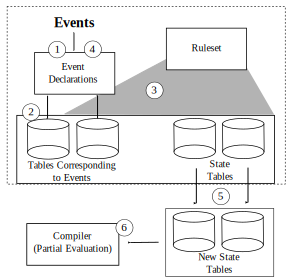
\includegraphics[scale=0.95]{figs/eval-cycle.pdf}
\caption{\small \flowlog's workflow for responding to events. The boxed portion of the diagram appeared as \Cref{fig:events}.}
\label{fig:workflow}
\end{figure}

Figure~\ref{fig:workflow} sketches the controller's workflow. When an event
arrives (1) the controller converts it into a tuple and places it in the appropriate
input table via XSB's \fl{assert} command (2). Then, for each
outgoing and state-modification table, the controller queries XSB to obtain a set
of outgoing tuples (3) which are converted to events (4). Then each state-modification
tuple is \fl{asserted} or \fl{retracted} to result in the new state (5).
Finally, proactive compilation (6) is performed on the new state,
producing a NetCore policy. 

\paragraph{External Events}

\flowlog\ evaluation is triggered by a general set of events; the runtime must watch
for more than just packet arrivals.
For instance, the runtime sends an event to the controller whenever a switch
registers or goes down, and as seen in Section~\ref{sec:examples}, external
applications may also interact with \flowlog\ through events. Our hypothetical
campus police-officer informs \flowlog\ to register a stolen laptop by
using a small application (around 100 lines, most of which is boilerplate) that uses
Thrift to send an asynchronous message to \flowlog.

\paragraph{Remote Tables and Caching}

\flowlog\ rules reference a database of relational facts. As seen in
Section~\ref{sec:syntax}, tables can be declared either as local or remote. A
local table is managed internally by the controller (via \fl{assert} and
\fl{retract} statements to XSB), while a remote table is merely an
abstraction over callouts to external code. Like events,
these callouts use Thrift RPC to interact with external code. Unlike
events, callouts are synchronous. Callouts have the form of an ordinary state-referencing
formula, $R(t_1, ..., t_n)$, but each $t_i$ must be either a constant value or
a variable. After \flowlog\ queries the correct external
application, the reply contains a set of tuples of constants---one constant for
each variable in the query.
 
Although the rules see no distinction between local and remote
tables, in practice it would be impractical or impossible
to obtain \emph{entire} remote tables (such as an infinitely large
table that represents the addition of numbers).
Therefore, \flowlog\ obtains tuples from external
code only when they are needed by a rule. 
A na{\"i}ve implementation could simply obtain remote tuples
every time they were required; however, that would mean forwarding rules could not
be compiled if they referred to external code. Instead, we cache remote tuples
for the declared time-to-live. Since we
maintain the remote cache in XSB, when it comes time to react to an event, the
controller handles remote and local state in exactly the same way: via XSB.

When an event arrives, we invalidate cached tuples whose time-to-live has expired.
If the expired tuples were used in a compiled policy, we force an
update of the cache and provide switches with the new policy.
External programs are expected to not update their internal state or otherwise
provide inconsistent results within the \fl{TIMEOUT} values of their \flowlog\ definitions.

\paragraph{Handling Overlapping Rules}

In some SDN applications, switches will forward a packet on the
data plane and also send it to the controller. If we kept the pre-compilation
ruleset unmodified on the controller, this could lead to packet duplication
due to the compiled forwarding rules:
packets would be forwarded once by the switch tables, and forwarded again by
the same rule's action on the controller.

Since the compilability of a rule is independent of controller state, we can
determine which rules these are at program startup. We then leave these rules
out of what we pass to XSB, and disallow the controller from taking duplicate
actions. However, since there is a delay between the controller's state change
and corresponding rules being installed on the switches, this is not a perfect
solution: packets may be in-transit during deployment of the new policy. This
issue is not unique to \flowlog, and has been noted by
others~\cite{reitblatt:sigcomm12-consistent-updates}.

\paragraph{Performance and Scalability}

\flowlog\ is proactively compiled to switch rules whenever
possible. From the traffic
forwarding perspective, therefore, \flowlog\ is largely dependent on what is
supported in switch hardware.
We have confirmed experimentally that, as one would hope, the controller
receives no unnecessary packets. For instance, a \flowlog\ learning switch
never sends the controller a packet once that packet's source location is 
learned, and eventually the controller is not burdened at all. Packet-counts
were confirmed by both {\tt ifconfig} counters
and packet events seen by \flowlog. We used {\tt ping}
packets and a Mininet~\cite{lantz++:hotnets10-mininet}-hosted virtual network to simulate network traffic.
We tested on tree topologies with $3$ and $7$ switches
as well as a cyclic $3$-switch topology to test controller robustness, and have begun
testing on larger topologies as well.

Because forwarding in \flowlog\ is as fast as hardware allows, 
one scalability question remains:
since \flowlog\ compiles the controller state into NetCore
policies, how does this scale as the controller's
database grows?
The size of the NetCore policy we produce depends on how table references appear in the ruleset. 
The compiler produces a policy fragment for each rule, whose size is
proportional to the number of clauses generated by partial evaluation
(Section~\ref{sec:comp-partial}). Partial evaluation replaces state table
references in each rule with the disjunction of every matching tuple in that
table.
The largest number of 
clauses produced by a rule that references tables $R_1$ through $R_k$ is
$|R_1| \times \cdots \times |R_k|$,
which is the best achievable in the worst case. (This ensues
because we don't need to lift negated disjunctions, a technical detail that we lack
space to describe.)
We also simplify the resulting policies, which further
reduces their size in practice.
To convert policies to flow-table rules, we rely upon NetCore's
optimizing compiler~\cite{monsanto:popl12-netcore}.

To evaluate the quality of the NetCore policies our compiler produces,
we ran a \flowlog\ learning-switch program, using {\tt dpctl
dump-flows} to count the maximum number of table entries it produced on per
switch. We then did the same with the 
OCaml learning-switch module
in the Frenetic repository.
The Frenetic example produced a maximum of 25 rules per switch for the
3-switch tree and 81 rules per switch for the 7-switch tree. Our program
initially produced 40 rules and 108 rules respectively. The increased number
of rules was because \flowlog\ did not make use of OpenFlow's built-in flood
action, whereas the OCaml program did. After adding an optimization to our
learning-switch program that forced the use of the flood action, we saw the
same number of table entries as with the Frenetic version.
This indicates that our compiler can match the scalability of existing programs that use NetCore.

%%%%%%%%%%%%%%%%%%%%%%%%%%%%%%%%%%%%%%%%%%%%%%%%%%%%%%%%%%%%%%%%%
%%%%%%%%%%%%%%%%%%%%%%%%%%%%%%%%%%%%%%%%%%%%%%%%%%%%%%%%%%%%%%%%%


\section{Related Work}
\label{sec:rw}

\begin{table*}
\small
\begin{center}
\begin{tabular}{|l|l|c|c|c|c|c|c|}
  \hline
  {\bf Language}                          & {\bf Type} & {\bf State} & {\bf Rec?} & {\bf Neg?} & {\bf Compilation} & {\bf Reasoning?} & \bf{Callouts} \\
  \hline\hline
  Flog~\cite{katta:xldi12-flog}           & Rule-Based & \ck         & \ck        & \xm        & Reactive          & \xm                 & \xm  \\ \hline
  FML~\cite{hinrichs:wren09-fml}          & Rule-Based & \ck         & \xm        & \ck        & Reactive          & \xm                 & \xm  \\ \hline
  Frenetic~\cite{foster:icfp11-frenetic}  & FRP        & \cpo        & \xm        & \ck        & Reactive          & \xm                 & \xm  \\ \hline
  Frenetic OCaml Environment              & Functional & \cpl        & \cpl       & \ck        & via NetCore       & \xpl                & \cpl \\ \hline
  NetCore~\cite{monsanto:popl12-netcore}  & DSL        & \xm         & \xm        & \ck        & Proactive         & \ck                 & \xm  \\ \hline
  Nlog~\cite{koponen++:nsdi14-vmware-nlog}       & Rule-Based & \ck         & \xm        & \xm        & Proactive         & \xm                 & \ck  \\ \hline
  NOX~\cite{gude:ccr08-nox}               & Imperative & \cpl        & \cpl       & \ck        & Manual            & \xpl                & \cpl \\ \hline
  Procera~\cite{voellmy:hotsdn12-procera} & FRP        & \ck         & \xm        & \ck        & Unclear           & \xm                 & \xm  \\ \hline
  Pyretic~\cite{monsanto++:nsdi13-pyretic}& Imperative & \cpo        & \cpl       & \ck        & Proactive              & \xm                 & \cpl \\ \hline
  \hline
  \flowlog                                & Rule-Based & \ck  & \xm  & \ck  & Proactive   & \ck & \ck  \\
  \hline
\end{tabular}
\end{center}
\caption{\small SDN language comparison. {\bf Rec?} and {\bf Neg?} mean 
recursion and negation, respectively. A \ck\ means that a feature is present
and a \xm\ that it is not;
\cpl\ denotes that a feature's presence is due to embedding in a Turing-complete programming
language. In the {\bf State?} column,
\cpo\ indicates that maintaining a stateful forwarding policy is possible, but
that general state requires wrappers in a Turing-complete language. In the
{\bf Reasoning?} column, a \xpl\ indicates that \emph{sound} reasoning is made
non-trivial by Turing-completeness, and a \xm\ means that verification has not
been attempted.}
\label{tab:relwork}
\hrule
\normalsize
\end{table*}

Our work here draws on a prior workshop
paper~\cite{ngdfk:hotsdn13-flowlog}. The previous version mentioned,
yet did not describe or implement, external events and state. Our
proactive compiler, conversion to Alloy, topology-independent
verification, and implementation are also new. We compare other SDN
programming languages side-by-side with \flowlog\
in~\Cref{tab:relwork}, and discuss each in detail below.

FML~\cite{hinrichs:wren09-fml} provides a
stateful, rule-based idiom for forwarding policies.  It too
disallows recursion and admits negation. FML can read from, but not
modify, the underlying system state. It responds to new flows reactively,
whereas \flowlog\ proactively compiles to switch tables whenever possible. FML
does not provide abstractions for external code, and does not
address verification.

Frenetic~\cite{foster:icfp11-frenetic} is a functional-reactive (FRP) language that 
responds to fine-grained network events. While Frenetic was originally 
reactively compiled, it has since been extended with proactive compilation for stateless
NetCore~\cite{monsanto:popl12-netcore} policies. State and interaction with
external code must be managed by OCaml wrapper applications.
Frenetic also includes switch-based events and rich query constructs;
\flowlog\ lacks abstractions for queries, yet provides more general events.
Verification of full Frenetic
programs has not been addressed, although Gutz, et al.~\cite{gutz:hotsdn12-slices} use model-checking to 
prove slice isolation properties of NetCore policies.
Our runtime is currently implemented atop Frenetic's OCaml library and uses NetCore's optimizing compiler.
Guha et al.~\cite{guha:sdnverif} have created a verified compiler for a subset of NetCore; our compiler has
only been tested, not proven correct.

Pyretic~\cite{monsanto++:nsdi13-pyretic} implements NetCore~\cite{monsanto:popl12-netcore} in Python,
and introduced sequential composition of network programs.
Though we do not address program
composition explicitly, sequential and parallel composition are roughly
analogous to \flowlog's relational join and union, respectively.
Since its initial publication, Pyretic has been extended with proactive compilation.
Verification of Pyretic programs has not been discussed.

Flog~\cite{katta:xldi12-flog} is stateful and rule-based. It allows recursion
but not explicit negation in rule bodies; negation is implied in some cases by
rule-overriding. Flog has no notion of callouts or external events unrelated
to packets, and the paper does not address verification. Flog works at the
microflow level, whereas \flowlog\ is proactive.

Procera~\cite{voellmy:hotsdn12-procera} is another
FRP SDN language. As Procera is embedded in Haskell, programs have access to
general state and external callouts. Procera allows
programs to react to external events, but does not directly support
issuing events or external queries. Like Frenetic, Procera
provides query functionality that \flowlog\ does not. To
our knowledge, Procera programs have not been verified, and it
is unclear whether the flow constraints they generate are proactively compiled.

Nlog~\cite{koponen++:nsdi14-vmware-nlog}, a rule-based
configuration language, is part of a larger project on network
virtualization. When system state changes, an Nlog program dictates a new
virtual forwarding policy. Nlog's inability to modify controller
state means that it is not ``tierless''. Like \flowlog, Nlog is also proactively compiled
to flow tables, and our relational abstraction for callouts is similar to Nlog's. 
Verification of Nlog programs has not been discussed.

Maple~\cite{voellmy:sigcomm13-maple} is a controller platform that unifies control-
and data-plane logic; \flowlog\ goes further by also integrating controller state,
creating a tireless abstraction. Unlike in \flowlog, Maple programs are compiled
reactively, and have not been verified.

%%%%%%

A number of other rule-based languages also merit discussion, although
they were not built for SDNs and do not compile to flow tables. 
NDLog~\cite{loo:commacm09-declarative-networking} and OverLog~\cite{blt+:sosp05-overlog} are
declarative, distributed programming languages. In these languages, each tuple in the
relational state resides on a particular switch.
This is in contrast to the single controller state assumed by
\flowlog. These languages support recursion as in ordinary Datalog. Wang, et
al.~\cite{wang+:padl09-declarative-network-verif} verify NDLog programs via
interactive theorem provers, and some of the properties they verify are
topology-independent. Our compiler to Alloy requires far less user
effort and is simplified by \flowlog's lack of recursion. 
Alvaro, et al.~\cite{alvaro:datalog10-dedalus} present Dedalus, a variant of
Datalog with a notion of time. Our treatment of state change
is similar to theirs, except that theirs is complicated by recursion. 
Active networking~\cite{tennenhouse:ieeecommmag97-activenetworks} is a
forerunner of SDN where packets carry programmatic instructions for switches.
Like SDN, active networking has inspired language design efforts. One such is
ANQL~\cite{rogers:iwan02-anql}, a SQL-like language for defining packet
filters and triggering external code. \flowlog\ echoes ANQL's view of packets
as entries in a database, but supports more general external
stimuli. Verification of ANQL has not been discussed.

%\flowlog\ adopts what they aptly refer to as a ``chain of fixpoints'' semantics.

There is also a rich landscape of related SDN verification. Canini, et
al.~\cite{canini:nsdi12-nice} find bugs in Python controller
programs. Their work required the creation of a purpose-built model-checker.
Although their tool successfully finds bugs, it is limited by the
undecidability of Python code analysis. \flowlog's expressivity is
deliberately limited to avoid this concern. Skowyra et
al.~\cite{skowyra:hicons13} use model-checking to find bugs in SDN programs
sketched in their prototyping language, but focus solely on verification, not execution. Other reasoning
tools~\cite{alshaer:safeconfig10-flowchecker,gutz:hotsdn12-slices,khurshid:hotsdn12-veriflow,mai:sigcomm11-anteater,porras:hotsdn12-fortnox,xie:infocom2005-reachability}
analyze a fixed, stateless forwarding policy, either statically or at runtime.
Including transitions between states, as we do, is necessarily more complex.

\section{Discussion and Conclusion}
\label{sec:discussion}

To our knowledge, \flowlog\ is the first tierless SDN programming language,
the first stateful rule-based language for SDNs that proactively compiles to
flow-table rules, and the first such language to provide rich interfaces to
external code. Tierlessness simplifies the process of SDN programming and
simultaneously enables cross-tier verification of the SDN system.

Since tierlessness precludes manual handling of flow-table rules, automatic
flow-table management is necessarily a key part of any tierless SDN language.
There are other such strategies besides proactive compilation; a prototype
version of \flowlog\ simply sent all packets to the controller. However, a
proactive approach minimizes controller interaction and thus shows that a
tierless language can be performant.

In order to support efficient, proactive compilation and verification, we opted
to limit \flowlog's expressive power. Even with these limitations, we have built non-trivial
applications. Moreover, events and remote tables
allow \flowlog\ programs to access, when necessary, external code in languages
of arbitrary power.

%Rule-based programming is well-established in everything from configuration languages to
%SQL queries. It encompasses a broad range of expressive power. 
%\flowlog\ takes a somewhat extreme position by banning
%recursion. We justify this as follows:
%\begin{itemize}
%
%\item We have been able to build non-trivial applications without this
%  power. This limitation is an \emph{experiment} in how far we can push this
%  non-recursive style. By limiting its power, we exploit the same strengths as other
%  restricted languages like SQL, regular expressions, and context-free
%  grammars. 

%\item Despite this limitation, ``recursion'' can be obtained in other
%  ways. For instance, Section~\ref{sec:eg:nib} shows how a type of
%  transitive closure can be implemented without 
%  linguistic recursion. Therefore, this limitation is less
%  constraining than it seems.

%\item \flowlog\ programs are, by design, not closed systems.
%  It is therefore easy to communicate with computations of
%  arbitrary power. Indeed, \flowlog\ can reuse
%  existing code written in a variety of languages through simple shims
%  that treat them as producers and consumers of events or
%  tables. Therefore, the primary experiment is in whether the greater
%  power can go on the ``inside'' rather than on the ``outside''.

%\item In return for limiting the expressive power of the ``outside'',
%  we obtain two important strengths:
%
%  \begin{enumerate}
%
%  \item A powerful proactive compiler.
%
%  \item Richer verification support than most other languages
%    provide.
%
%  \end{enumerate}

%\end{itemize}

\paragraph{Future Work}

It is possible to strengthen \flowlog\ without abandoning our limitations on
expressive power. We plan to migrate to a newer version of OpenFlow soon,
which removes several uncompilable constructs in \Cref{tab:no-compile}. 
\flowlog's general event framework could support a query system like that seen in
Frenetic~\cite{foster:icfp11-frenetic} and other languages.
\flowlog's relational idiom supports the addition of new features. For instance, we have 
recently added address masking (e.g., matching packets coming from \fl{10.0.0.0/24}) to \flowlog\ by 
taking advantage of the fact that masks are simply relations over IP addresses. 

There are also several promising directions to take verification in \flowlog. 
For instance, we suspect that \flowlog's restrictions
could enable the sound and complete use of techniques like symbolic execution
for verifying trace properties.
Another important analysis, change-impact---which describes the
\emph{semantic} consequences of a program change---is undecidable for
general-purpose languages, yet is decidable for \flowlog.
